\documentclass[a4paper,12pt]{article}
\usepackage[left=2cm,top=2cm,right=2cm]{geometry}
\usepackage{fancyhdr}
\usepackage{graphicx}
\usepackage[utf8]{inputenc}


\title{Design Analysis}
\author{Group Project 3 - Group 2}
\date{March 21 2008}

\begin{document}
\maketitle
\newpage
\tableofcontents
\newpage



\section{Introduction}
This class diagram highlights the classes discovered during the analysis,
and some additional classes discovered during the design of our application.
You will notice than there is no methods in our classes related to the reading,the creation, the deletion or tu updating.
There is no such method because we assume that thoses features are handled from the roots by the GRails Framework.

\section{Class diagram}
\begin{figure}[htbp]
\begin{center}
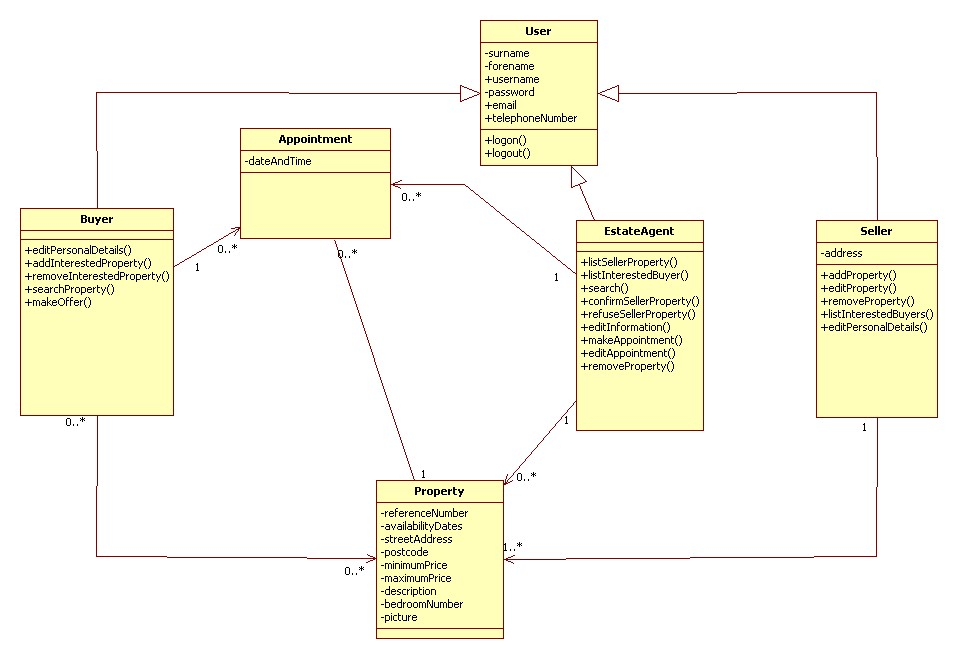
\includegraphics[width=\linewidth]{pics/classDiagram.jpg}
\end{center}
\caption{\footnotesize Class Diagram of Napier Estate Agency}
\end{figure}
\subsection {Classes description}

\subsubsection{EstateAgent class}
An estate agent inherits from an User.
He can :
\begin{itemize}
\item List his properties
\item List the buyers interested by his properties
\item Search a property
\item Validate (or not) a property in order to make it available on the website.
\item Edit the details of a property
\item Set up an appointment
\item Edit an appointment
\item Remove a property
\end{itemize}

\subsubsection{Buyer class}
A buyer inherits from an User.
He can :
\begin{itemize}
\item Add a property to his list of interests
\item Remove a property from this list
\item Search for a property
\item Make an offer to a property
\end{itemize}

\subsubsection{Seller class}
A seller inherits from an User.
He can :
\begin{itemize}
\item Add his property to the website (which is going to be validated by an estate agent)
\item See the list of buyers interested by his properties
\end{itemize}

\subsubsection{User class}
The Seller class, the Buyer class and the EstateAgent class have some common attributes and behaviors,
that's why a parent class, User, as been created to generalize theses attributes and behaviors.
An user is characterized by :
\begin{itemize}
\item His surname
\item His forename
\item A password
\item An email
\item His telephone number (should be formatted like an UK number)
\end{itemize}
This class handles also the login and the logout of an user.

\subsubsection{Property class}
This class describe a property. A property is characterized by : 
\begin{itemize}
\item A reference number (Unique identifier for a property)
\item A set of availability dates
\item A postcode (constrained by the UK Postcode format)
\item A minimum price
\item A maximum price
\item A short description of the property
\item The number of bedrooms
\item A set of pictures
\end{itemize}

\subsubsection{Appointment class}
This class describes an appointment, set at a particular date and a particular time.
Constraint : A estate agent or a buyer can't have more than one appointment same date.



\section{Use-Case Diagram}

\subsection{Napier Estate Agency use case diagram}
\begin{figure}[htbp]
\begin{center}
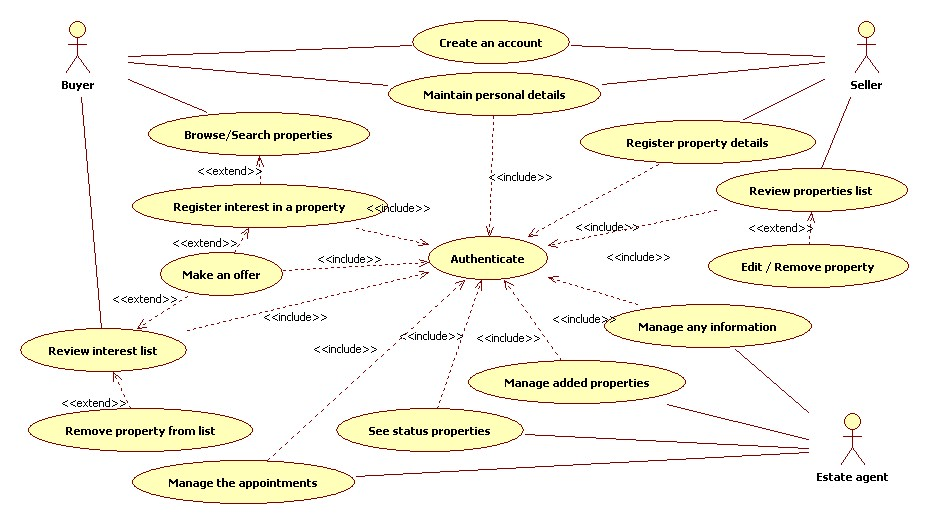
\includegraphics[width=\linewidth]{pics/useCases.jpg}
\end{center}
\caption{\footnotesize Use-Case Diagram of Napier Estate Agency}
\end{figure}


\section{Use-Case Specification}

\subsection{Authenticate}

The user logs on to the website to benefit of its services which are provided by the website.

\paragraph{Basic Flow}
\begin{enumerate}
\item The system prompts the user to log on.
\item The user enters his username and password.
\item The system verifies the logon information.
\item The system logs user on to system.
\end{enumerate}
\paragraph{Alternative Flow}
\begin{enumerate}
\item The system recognizes cookie on user's machine. 
\item Go to step 4 (Basic Flow).
\item The system does not recognize user's logon information.
\item Go to step 1 (Basic Flow).
\end{enumerate}
\paragraph{Pre-Conditions}
The user has to want to use a service other than "browse properties", "create an account".
\paragraph{Post-Conditions}
The user will enjoy all the services whose he is allowed to use.

\subsection{Browse/Search properties}

The buyer can search properties by location or postcode and concequentely browse all the referenced properties in the website's database.

\paragraph{Basic Flow}
\begin{enumerate}
\item The system shows the list of all properties available.
\item The buyer enteres in the engine search some filters such as the postcode.
\item The system provides an reply from the buyer's request in displaying a new list.
\end{enumerate}
\paragraph{Alternative Flow}
\begin{enumerate}
\item The system shows the list of all properties available.
\item The user can switch the part's list of properties in clicking on directional arrows.
\end{enumerate}
\paragraph{Post-Conditions}
The buyer finds porperties which match to his searches.

\subsection{Create an account}

To create a new account object with personal details, including name, contact number and address.

\paragraph{Basic Flow}
\begin{enumerate}
\item The system prompts the user for his forename, surname, his contact number, and his address.
\item If the user does not exist previously in the database, and if the data is validated, the sytem add the new record.
\item The user is logged-on directly on his new account.
\end{enumerate}
\paragraph{Alternative Flow}
\begin{enumerate}
\item
\end{enumerate}

\subsection{Edit / Remove property}

The seller can update properties information if he did some mistakes. He can also remove its properties if the Napier Agency's contract allows him to use this use case.

\paragraph{Basic Flow}
\begin{enumerate}
\item The seller changes any information about his property.
\item The system verifies the data's type entered.
\item The system processes the modifications on the database.
\end{enumerate}
\paragraph{Pre-Conditions}
The seller must be log on the system.
\paragraph{Post-Conditions}
The modifications wanted by the seller are done.

\subsection{Maintain personal details}

The seller and the buyer maintain their personal details online either edit or remove information.

\paragraph{Basic Flow}
\begin{enumerate}
\item The seller or the buyer change any information about his personal details.
\item The system verifies the data's type entered are allowed.
\item The system processes the modifications on the database.
\end{enumerate}
\paragraph{Pre-Conditions}
The seller and the buyer must be log on the system.
\paragraph{Post-Conditions}
The personal information are modified and saved in the system.

\subsection{Manage added properties}

The estate agent checks, confirms and refuses all the added properties by the sellers. By this way he still keeps the control in order to obtain consitent data.

\paragraph{Basic Flow}
\begin{enumerate}
\item The system prompts a list of properties to be validated.
\item The estate agent chooses a property to validate.
\item The system prompts the property details and ask for a confirmation.
\item The estate agent chooses to validate the property.
\item The system markes the property as validated.
\end{enumerate}
\paragraph{Alternative Flow}
\begin{enumerate}
\item The user chooses to not validate the property.
\item The property is deleted.
\end{enumerate}
\paragraph{Pre-Conditions}
The estate agent must be logged on the system.


\subsection{Manage any user information}

Any user can change his credential, or delete his own account.

\paragraph{Basic Flow}
\begin{enumerate}
\item
\end{enumerate}
\paragraph{Alternative Flow}
\paragraph{Pre-Conditions}
The estate agent must be log on the system.

\subsection{Manage the appointments}

The estate agent arranges the appointments for people who want visit properties.

\paragraph{Basic Flow}
\begin{enumerate}
\item The estate agent asks the system to process a new appointment.
\item The system asks the estate agent for identification.
\item The estate agent identifies himselve to the system.
\item The system displays a list of buyers interested by properties to the estate agent.
\item The estate agent selects the buyer and his interested property into the system.
\item The system displays the diary with the date available for a visit to the sales assistant.
\item The estate agent chooses a date.
\item The system displays the appointment's description created by the estate agent.
\item The estate agent valids his appointment.
\item The system records the appointment.
\item The system removes the choosen date for the appointment from date available.
\item The system displays the main menu to the estate agent.
\end{enumerate}
\paragraph{Alternative Flow}
\begin{enumerate}
\item The system recognizes cookie on estate agent's machine. 
\item Go to step 4 (Basic Flow).
\item The system does not recognize estate agent's logon information.
\item Go to step 2 (Basic Flow).
\end{enumerate}
\paragraph{Pre-Conditions}
The system is displaying the estate agent main menu.
\paragraph{Post-Conditions}
The system is displaying the estate agent main menu.

\subsection{Register interest in a property}

To makes an offer online and wait for result/notice from agent after deadline.

\paragraph{Basic Flow}
\begin{enumerate}
\item
\end{enumerate}
\paragraph{Pre-Conditions}
The buyer must be log on the system.

\subsection{Register property details}

The seller adds a new property in gathering the key features, full description, tenure and in uploading pictures.

\paragraph{Basic Flow}
\begin{enumerate}
\item The seller asks the system to process a new add property.
\item The system asks the seller for identification.
\item The seller identifies himselve to the system.
\item The system displays a blank dossier of add property to the seller.
\item The seller fills all the required fields with the features of his property and uploads pictures of his property into the system.
\item The system displays the description of request's seller to the seller.
\item The seller valids his add.
\item The system records the property details.
\item The system signals to an estate agent that a property of the seller has been added and has to be confirmed.
\item The system displays the seller main menu to the seller.
\end{enumerate}
\paragraph{Alternative Flow}
\begin{enumerate}
\item The system recognizes cookie on seller's computer. 
\item Go to step 4 (Basic Flow).
\item The system does not recognize seller's logon information.
\item Go to step 2 (Basic Flow).
\end{enumerate}
\paragraph{Pre-Conditions}
The system is displaying the seller main menu.
\paragraph{Post-Conditions}
The system is displaying the seller main menu.

\subsection{Remove property from list}

The buyer removes a property from the basket if he is not interested by one added property.

\paragraph{Basic Flow}
\begin{enumerate}
\item The buyer asks the system to remove a property.
\item The system asks the buyer for identification.
\item The seller identifies himselve to the system.
\item The system checks if an appointment is arranged between the buyer and an estate agent.
\item The system remove the property from the buyer's basket.
\item The system prints the basket without the property which was just removed to the buyer.
\end{enumerate}
\paragraph{Alternative Flow}
\begin{enumerate}
\item The system recognizes cookie on buyer's computer. 
\item Go to step 4 (Basic Flow).
\item The system does not recognize buyer's logon information.
\item Go to step 2 (Basic Flow).
\end{enumerate}
\paragraph{Pre-Conditions}
The system is displaying the buyer main menu.
\paragraph{Post-Conditions}
The system is displaying the buyer basket.

\subsection{Review interest list}

The buyer see the interested properties in his basket in order to check back his favours next sign in.

\paragraph{Basic Flow}
\begin{enumerate}
\item The buyer asks the system to list its interested properties.
\item The system asks the buyer for identification.
\item The buyer identifies himselve to the system.
\item The system prints the list of properties which were added by the buyer in the basket.
\end{enumerate}
\paragraph{Alternative Flow}
\begin{enumerate}
\item The system recognizes cookie on buyer's computer. 
\item Go to step 4 (Basic Flow).
\item The system does not recognize buyer's logon information.
\item Go to step 2 (Basic Flow).
\end{enumerate}
\paragraph{Pre-Conditions}
The buyer must be log on the system.


\subsection{Review properties list}

The seller see his added properties list.

\paragraph{Basic Flow}
\begin{enumerate}
\item The seller asks the system to list its properties.
\item The system asks the seller for identification.
\item The seller identifies himselve to the system.
\item The system displays the list of all properties belong to his owners.
\end{enumerate}
\paragraph{Alternative Flow}
\begin{enumerate}
\item The system recognizes cookie on seller's computer. 
\item Go to step 4 (Basic Flow).
\item The system does not recognize seller's logon information.
\item Go to step 2 (Basic Flow).
\end{enumerate}
\paragraph{Pre-Conditions}
The seller must be log on the system.
\paragraph{Post-Conditions}
The seller see the inventory of his properties.

\subsection{See status properties}

The estate agent see who are interested by properties and also the name of its owners.

\paragraph{Basic Flow}
\begin{enumerate}
\item The system displayes the list of all buyer who are interested by properties.
\item The estate agent get more details in clicking on the properties.
\item The system displayes all the details buyer, property, seller.
\end{enumerate}
\paragraph{Pre-Conditions}
The estate agent must be log on the system.
\paragraph{Post-Conditions}
The estate agent see the dossier of each property which has been selected by buyers.


\end{document}
